\blueheader
\begin{frame}
\frametitle{1C: Aritmetisk rekke }

\begin{blue*}{Definisjon}
En \textbf{aritmetisk rekke} er en rekke der differansen mellom påfølgende ledd er konstant $d$:
\begin{equation*}
a_{n+1} = a_n + d \quad \text{for } n \ge 1.
\end{equation*}
Tallet $d$ kalles \emph{differansen}.
\end{blue*}

\begin{cyan*}{Oppgave}
Hvordan kan vi undersøke om en følge er aritmetisk?

\end{cyan*}

\end{frame}

\blueheader
\begin{frame}
\frametitle{1C: Det n-te leddet i en aritmetisk rekke}

\begin{red*}{Regel}
Det $n$-te leddet i en aritmetisk rekke med differanse $d$ er gitt ved
\[
a_n = a_1 + (n-1)\,d.
\]

(Bevist med induksjon i oppgave 1.66.)
\end{red*}

\end{frame}

\greenheader
\begin{frame}{1C: Eksempel (I)}
I en aritmetisk rekke er 
\[
a_{10} = 37 \quad \wedge \quad a_{16} = 61
\]
Finn en formel for det $n$-te leddet i rekka.

\medskip
Siden rekka er aritmetisk, får vi ledd nr. 16 ved å legge til 6 differanser til ledd nr. 10:
\[
a_{16} = a_{10} + 6d.
\]

Vi setter inn verdiene:
\[
61 = 37 + 6d \quad \Rightarrow \quad d = 4.
\]
\end{frame}

\greenheader
\begin{frame}{1C: Eksempel (II)}
Vi har nå funnet at $d=4$. Vi må nå finne en verdi for $a_1$.

\medskip
Generell formel for et ledd i en aritmetisk rekke er
\[
a_n = a_1 + (n-1)\cdot d
\]

Fra $a_{10} = 37 = a_1 + (10-1)\cdot d $ får vi
\begin{align*}
a_1 &= 37 - (10-1)\cdot 4\\ 
&= 1
\end{align*}

\medskip
Altså er formelen for rekka
\begin{align*}
a_n &= 1 + (n-1)\cdot 4\\ &= 4n - 3
\end{align*}
\end{frame}



\blueheader
\begin{frame}
\frametitle{1C: Summen til en aritmetisk rekke }

\begin{red*}{Regel}
Summen av de $n$ første leddene i en aritmetisk rekke er
\[
s_n = \frac{n}{2}\,(a_1 + a_n)
\]

Beviset står på side 48.
\end{red*}

\begin{red*}{En nyttig formel for summen som ikke bruker siste ledd i rekken}
Ved å sette inn $a_n = a_1 + (n-1)\cdot d$ får vi formelen:
\[
s_n = \frac{n}{2}\,\bigl(2a_1 + (n-1)\cdot d\bigr)
\]


\end{red*}

\end{frame}

%----------------------------------

\blueheader
\begin{frame}
\frametitle{1C: Geometrisk rekke}

\begin{blue*}{Definisjon}
En \textbf{geometrisk rekke} er en rekke der forholdet mellom påfølgende ledd er konstant:
\[
a_{n+1} = a_n \cdot k \quad \text{for } n \ge 1
\]

Tallet $k$ kalles \emph{kvotienten} til rekka.
\end{blue*}



\begin{cyan*}{Oppgave}
Hvordan kan vi undersøke om en følge er geometrisk?
\end{cyan*}

\end{frame}


\blueheader
\begin{frame}
\frametitle{1C: Geometrisk rekke}

\begin{red*}{Regel}
Det $n$-te leddet i en geometrisk følge med kvotient $k$ er gitt ved
\[
a_n = a_1 \cdot k^{\,n-1}
\]

(Bevis kan gjøres ved induksjon. Se side 52)
\end{red*}

\end{frame}

\blueheader
\begin{frame}
\frametitle{1C: Geometrisk rekke}

\begin{cyan*}{Oppgave}
Finn en formel for det $n$-te leddet i rekka
\[
2 + \tfrac{2}{3} + \tfrac{2}{9} + \tfrac{2}{27} + \ldots
\]

\begin{itemize}
    \item Startledd: 
    \item Finn kvotienten: 
    \item Bruk formelen $a_n = a_1 \cdot k^{\,n-1}$
\end{itemize}
\end{cyan*}

\end{frame}


\greenheader
\begin{frame}{1C: Eksempel}
I en geometrisk rekke er 
\[
a_6=405 \quad \wedge \quad a_{10}=32\,805
\]
Finn en formel for det n-te leddet.
\begin{center}
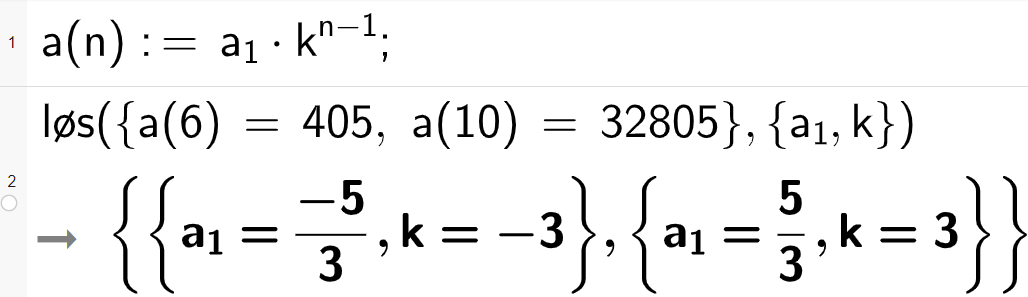
\includegraphics[width=0.6\textwidth]{R2K1C-1.png}
\end{center}
Vi får to mulige formler
\[
a_n=\frac{5}{2}\cdot 3^{n-1}\quad\wedge\quad a_n=-\frac{5}{2}\cdot (-3)^{n-1}
\]
\end{frame}


\redheader
\begin{frame}{1C: Summen av de $n$ første leddene i en geometrisk rekke}


Summen av de $n$ første leddene i en geometrisk rekke med
\begin{itemize}
    \item startledd $a_1$ \\
    \item og kvotient $k \neq 1$
\end{itemize}

\medskip
er gitt ved
\[
S_n = a_1 \cdot \frac{k^n - 1}{k - 1}.
\]

\medskip
Hvis $k=1$, er alle leddene like, og vi får
\[
S_n = n \cdot a_1.
\]
(Bevis står på side 52)
\end{frame}

\greenheader
\begin{frame}{1C: Eksempel (I)}
Finn summen av de ti første leddene i den geometriske rekka 
\[
729+810+900+1000+...
\]
Finner kvotienten
\[
\frac{1000}{900}=\frac{10}{9}
\]

\medskip
Summen av de $n$ første leddene er gitt ved
\[
S_n = a_1 \cdot \frac{k^n - 1}{k - 1}.
\]

\medskip
For $n=10$:
\begin{align*}
S_{10} &= 729 \cdot \frac{\left(\tfrac{10}{9}\right)^{10} - 1}{\tfrac{10}{9} - 1}\\
&= 12\,266,76
\end{align*}
\end{frame}

\greenheader
\begin{frame}[fragile]{1C: Eksempel (II)}
\begin{center}
\Large
\begin{verbatim}
sum(a(n),n,1,10)
\end{verbatim}
\end{center}

\begin{center}
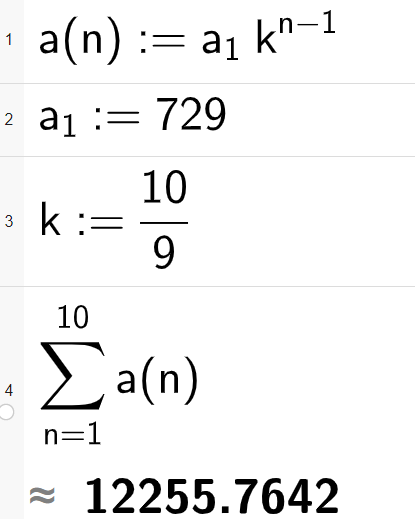
\includegraphics[width=0.3\textwidth]{R2K1C-2.png}
\end{center}
\end{frame}


\greenheader
\begin{frame}[fragile]{1C: Eksempel (III)}
\begin{minted}[fontsize=\footnotesize]{python}
a1 = 729            # Første ledd i den geometriske rekken
k = 10/9            # Kvotienten (hvor mye vi ganger med fra ett ledd til det neste)

minliste = []       # Vi starter med en tom liste

# Vi vil finne de 10 første leddene i rekken
for n in range(1, 11):                    # n går fra 1 til 10
    ledd = round(a1 * k**(n-1), 2)        # regner ut n-te ledd, avrundet til 2 desimaler
    minliste.append(ledd)                 # legger leddet inn i listen

print(minliste)
# Output:  
# [729.0, 810.0, 900.0, 1000.0, 1111.11, 1234.57,
#  1371.74, 1524.16, 1693.51, 1881.68]

# Beregner summen av alle leddene
summen = sum(minliste)
print(summen)
# Output: 12255.77
\end{minted}
\end{frame}

\begin{comment}
\greenheader
\begin{frame}[fragile]{1C: Eksempel (IV) løser ved å bruke list comprehension}
\warn
\begin{minted}[fontsize=\footnotesize]{python}
a1 = 729            # Første ledd i den geometriske rekken
k = 10/9            # Kvotienten (faktoren vi ganger med fra ett ledd til det neste)

# Lager en liste med de 10 første leddene i rekken med list comprehension.
# For hvert n fra 1 til 10 regner vi ut a1 * k^(n-1), og runder av til 2 desimaler.
minliste = [round(a1 * k**(n-1), 2) for n in range(1, 11)]

print(minliste)
# Output:
# [729.0, 810.0, 900.0, 1000.0, 1111.11, 1234.57,
#  1371.74, 1524.16, 1693.51, 1881.68]

# Regner ut summen av alle leddene i listen
summen = sum(minliste)
print(summen)
# Output: 12255.77

\end{minted}
\end{frame}
\end{comment}












